\section{Laboratorium IV}\label{sec:lab4}

\subsection{Wybrany sprzęt}\label{subsec:lab4-hw}

\emph{Enviro HAT} to~moduł zawierający pełny zestaw sensorów niezbędnych do~utworzenia małej stacji pogodowej.
Wykorzystuje standardowe wielofunkcyjne elementy wymienione w~tabeli~\ref{tab:enviromodules}.

\begin{table}[H]
  \caption{Układy scalone składające~się na~moduł \emph{Enviro}}
  \label{tab:enviromodules}
  \begin{tabularx}{\linewidth}{@{}lX@{}}
    \textbf{Układ} & \textbf{Opis} \\
    \midrule
    BME280         & Zawierający czujniki temperatury, ciśnienia, i~wilgotności. \\
    \midrule
    LTR-559        & Zawierający sensory jasności otoczenia i zbliżeniowy. \\
    \midrule
    SPH0645LM4H-B  & Mikrofon mikroukładowy \emph{I²S}. \\
    \midrule
    ST7735         & Sterownik wyświetlacza LCD $160\,\times\,80$ pikseli.
  \end{tabularx}
\end{table}

\subsection{Dodatkowe oprogramowanie}\label{subsec:lab4-sw}

Wykorzystanie sensorów w~kodzie jest~wzorowane na~bibliotece do~nowszej płytki \emph{Enviro+}\thinspace\cite{envirodoc}.
W~związku z~aktualizacją kodu tej~biblioteki z~\emph{Python~\num{2}} na~\emph{Python~\num{3}}, jej~struktura
nie~jest~zgodna z~najnowszymi rekomendacjami stylistycznymi, biblioteka skupia~się również w~głównej części na~sensorach
niedostępnych na~starszej wersji płytki w~posiadaniu uczelni.

W~trakcie pisania tej~pracy została również znaleziona i~zgłoszona niekompletność dokumentacji wymagań
modułu\thinspace\cite{enviroissue}.

W~związku z~tymi trudnościami kod laboratoriów wykorzystuje bardziej niskopoziomowe biblioteki i~reimplementuje
funkcjonalność dostępną w~oficjalnym źródle przy wykorzystaniu bibliotek wymienionych w~tabeli~\ref{tab:envirolibs}.

\begin{table}[H]
  \caption{Biblioteki języka \emph{Python} wykorzystane w~laboratorium IV}
  \label{tab:envirolibs}
  \begin{tabularx}{\linewidth}{@{}lX@{}}
    \textbf{Biblioteka} & \textbf{Opis} \\
    \midrule
    bme280      & Biblioteka wspierająca interakcje z~sensorami udostępnianymi przez~układ \emph{BME280}. \\
    \midrule
    ltr559      & Biblioteka wspierająca wykorzystanie sensorów układu \emph{LTR-559}. \\
    \midrule
    sounddevice & Standardowa biblioteka wykorzystywana do~interakcji z~urządzeniami audio w~języku Python,
                  w~tym~przypadku z~układem \emph{SPH0645LM4H-B}\@. \\
    \midrule
    st7735      & Biblioteka obsługująca wyświetlacz ciekłokrystaliczny \emph{ST7735}\@. \\
    \midrule
    font-roboto & Biblioteka dostarczająca rodzinę czytelnych czcionek \emph{Roboto} firmy Google do~wykorzystania
                  w~języku \emph{Python}. \\
    \midrule
    pillow      & Standardowa biblioteka \emph{Python} zawierająca funkcjonalności przetwarzania obrazów.
  \end{tabularx}
\end{table}

\subsection{Rozwiązanie}\label{subsec:lab4-sol}

Rysunek~\ref{fig:weatherlab} to~fragment instrukcji zawierający dwa~zadania.
Zadanie \emph{Z3.} wykorzystuje platformę \emph{ntfy.sh} do~wysłania powiadomienia w~momencie przykrycia czujnika
zbliżeniowego na~płytce, informacje zawarte w~tej wiadomości przedstawia rysunek~\ref{fig:weatherntfy}.
W~zadaniu \emph{Z4.} student wykorzystuje poprzednio uzupełnione funkcje do~złożenia pętli głównej obsługującej program
założony w~temacie laboratorium.

\begin{figure}[H]
  \centering
  \includegraphics[width=0.9\linewidth]{media/weather_lab}
  \caption{Fragment instrukcji IV}
  \label{fig:weatherlab}
\end{figure}

\begin{figure}[H]
  \centering
  \includegraphics[width=0.9\linewidth]{media/weather_ntfy}
  \caption{Powiadomienie pogodowe na platformie \emph{ntfy}}
  \label{fig:weatherntfy}
\end{figure}

Rysunek~\ref{fig:weather} przedstawia rozwiązanie zadania.
Program wyświetla kolejno zbierane dane wraz~z~wykresami wcześniejszych wartości.
Rysunek~ten jest~złożeniem dwóch zdjęć o~różnych ekspozycjach w~celu widoczności zarówno ekranu, jak~i~płytki,

\begin{figure}[H]
  \centering
  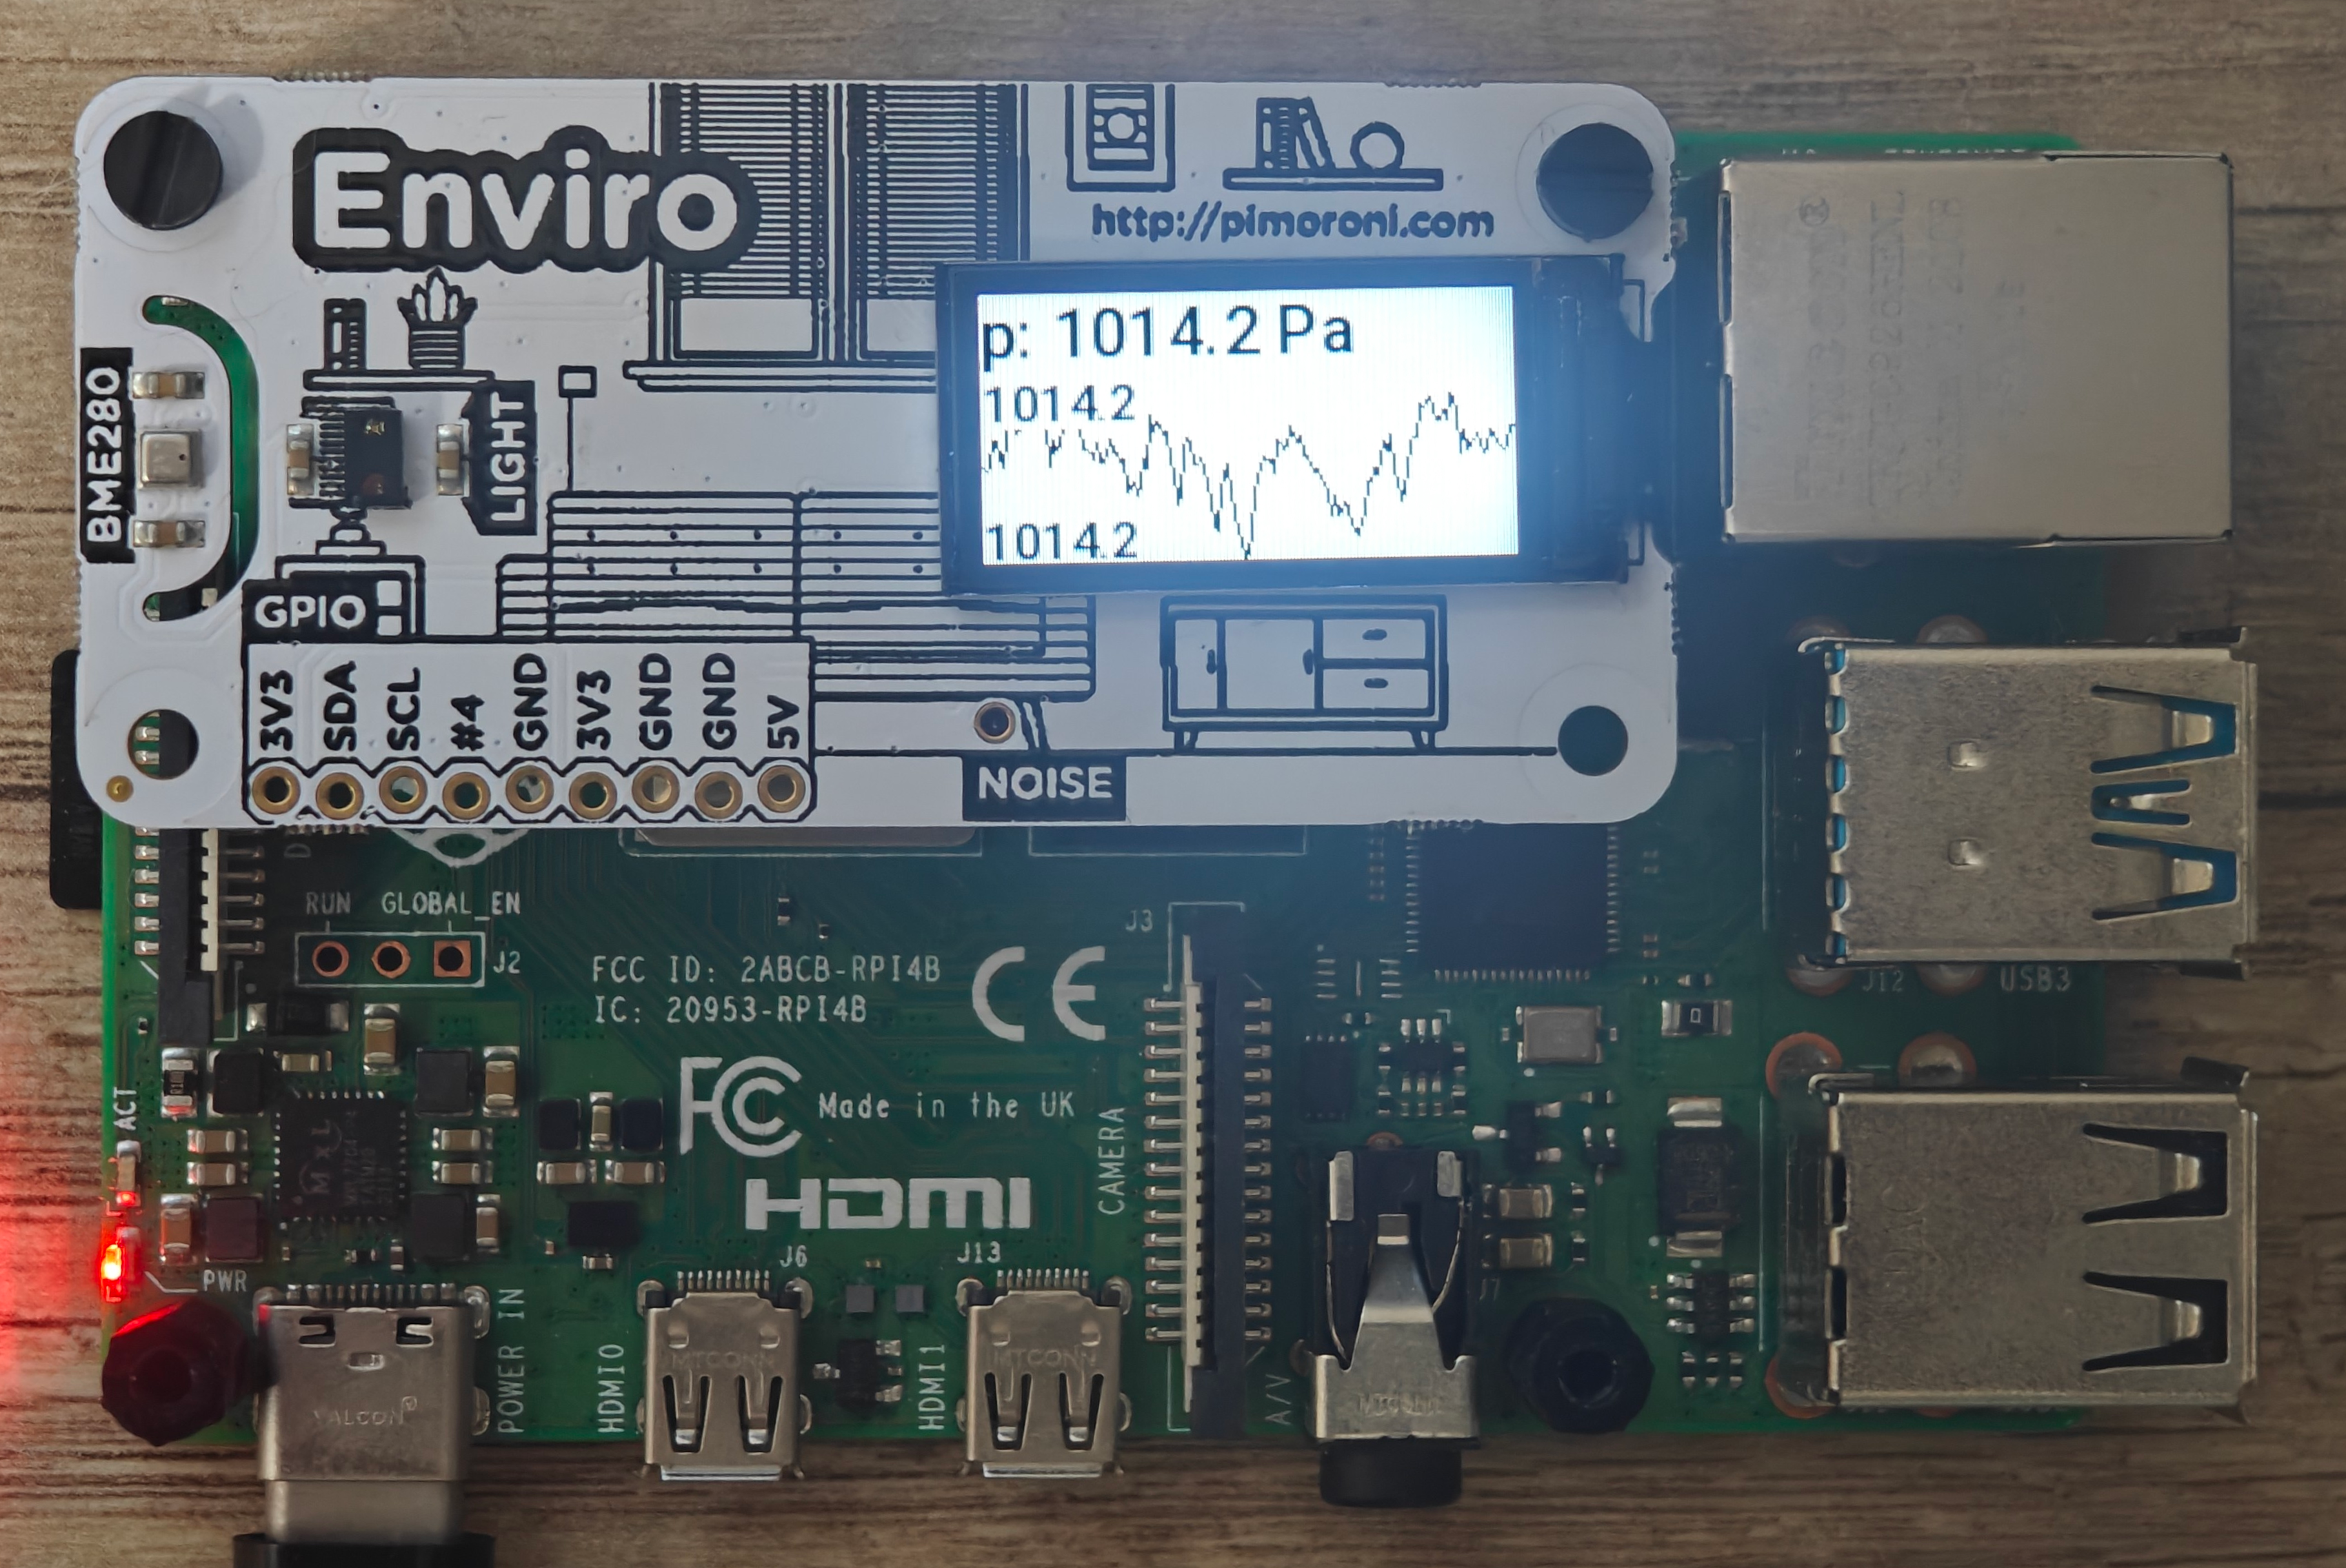
\includegraphics[width=0.6\linewidth]{media/weather}
  \caption{Uruchomiony program czwartego laboratorium}
  \label{fig:weather}
\end{figure}
